% Name: Stacked area plot
% Description: Electricity generation by source over a decade, each band stacked on the ones below so the top edge is the total.
% Tags: area plot, stacked, composition, time series

\usepackage{pgfplots}
\pgfplotsset{compat=1.18}

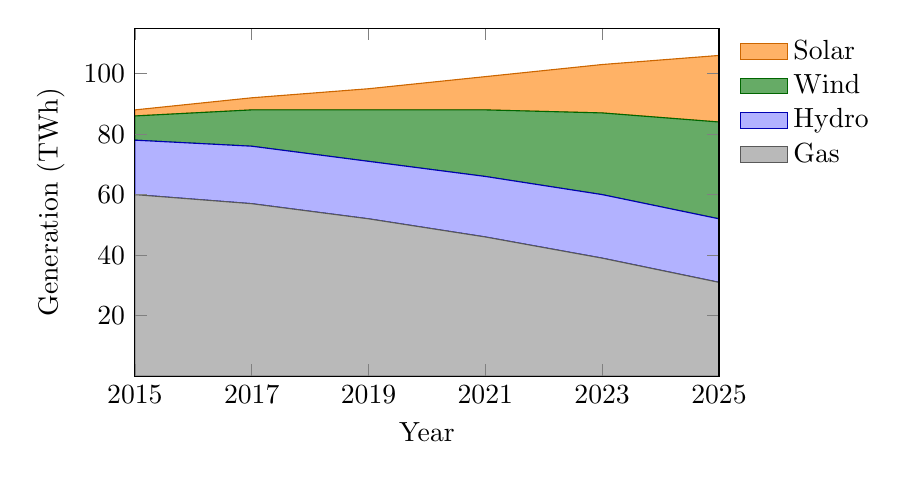
\begin{tikzpicture}
  \begin{axis}[
    width=9cm, height=6cm, stack plots=y, area style,
    xmin=2015, xmax=2025, ymin=0, ymax=115, ytick={20,40,...,100}, xtick={2015,2017,...,2025},
    x tick label style={/pgf/number format/1000 sep={}},
    xlabel={Year}, ylabel={Generation (TWh)},
    legend style={at={(1.02,1)}, anchor=north west, draw=none},
    reverse legend, legend cell align=left, axis on top,
  ]
    \addplot[fill=gray!55, draw=gray!70!black] coordinates {(2015,60) (2017,57) (2019,52) (2021,46) (2023,39) (2025,31)} \closedcycle;
    \addplot[fill=blue!30, draw=blue!70!black] coordinates {(2015,18) (2017,19) (2019,19) (2021,20) (2023,21) (2025,21)} \closedcycle;
    \addplot[fill=green!45!black!60, draw=green!40!black] coordinates {(2015,8) (2017,12) (2019,17) (2021,22) (2023,27) (2025,32)} \closedcycle;
    \addplot[fill=orange!60, draw=orange!80!black] coordinates {(2015,2) (2017,4) (2019,7) (2021,11) (2023,16) (2025,22)} \closedcycle;
    \legend{Gas, Hydro, Wind, Solar}
  \end{axis}
\end{tikzpicture}
